\chapter{Apresentação de Resultados}
\label{cap:avaliacao_sistema}

Nesse capítulo será feita a apresentação dos resultados obtidos a partir da aplicação do modelo proposto a um cenário.

%%%%%%%%%%%%%%%%%%%%%%%%%%%%%%%%%%%%%%%%%%%%%%%%%%%%%%%%%%%%%%%%%%%%%%%%%
\section{Introdução}

As discussões nesse capítulo estão descompostas em três partes, sendo elas:

\begin{itemize} \parskip -4pt
    \item \textbf{Fluxo de execução do sistema:} Apresenta a dinâmica do sistema a começar pela leitura dos produtos contidos na geladeira e finalizando na apresentação de recomendações e receitas, além de algumas funcionalidades dentre as descritas no Capítulo 4.
    \item \textbf{Cenário de Aplicação:} Apresenta o cenário através do qual o sistema será avaliado. Assim, detalha-se o ambiente da simulação, os dados utilizados, sua obtenção, organização além das ações executadas pelo sistema.
    \item \textbf{Avaliação do Protótipo:} Nesta seção, a partir do cenário proposto, serão demonstradas interações com o protótipo e o efeito gerado no sistema, seja na forma de recomendações de produtos e receitas, bem como em informações de estado da geladeira e de produtos contidos atualmente.
\end{itemize}

%%%%%%%%%%%%%%%%%%%%%%%%%%%%%%%%%%%%%%%%%%%%%%%%%%%%%%%%%%%%%%%%%%%%%%%%%
\section{Fluxo de execução do sistema}

No sistema diversas operações são executadas, às quais incluem os diversos componentes do sistema. A seguir, alguns fluxos de execução, dentre os mais relevantes, são apresentados e explanados.

% Demonstrar fluxo de execução da leitura de conteúdo
\subsection{Leitura de conteúdo}

No momento em que a geladeira for ligada, conforme a Figura \ref{fig:cap5_diagr_leitura}, o sistema será inicializado e as portas (ou terminais) serão configurados a fim de permitir a comunicação com os leitores além do mecanismo de fechamento. Ademais, os eventos, engatilhados pela mudança do estado da porta, também são configurados. Após a conclusão das ações mencionadas, o sistema entra em modo de espera.

A partir desse ponto, o sistema dependerá da ação do usuário para operar. Assim, quando o usuário abrir ou fechar a porta, o sensor fechamento irá propagar um novo sinal para o sistema. Quando tal evento de mudança ocorre, verifica-se qual o tipo de evento ocorreu, ou seja, entrada ou saída. Caso aberto, o sistema entra em modo de espera por alguns segundos, garantindo que a porta esteja realmente aberta e reduzindo as chances de ruídos interferirem no funcionamento do leitor. Além disso, garante-se que o usuário tenha tempo suficiente para fechar a porta de maneira voluntária. 

Após o período transcorrer, uma nova leitura é realizada e caso ainda aberta, um registro de porta aberta é enviado ao servidor. 

Caso for verificado, após a interação do usuário, que a porta está fechada, espera-se também alguns segundos. Após esse tempo, um comando de leitura é enviado para os leitores de etiquetas. Estes, por sua vez, realizam a captura das informações das \textit{tags} ao alcance e as enviam ao Raspberry. Por fim, um registro de interação é engatilhado no servidor e gravado na base de interações.

\begin{figure}[htb]
    \caption{Leitura de conteúdo da geladeira}
    \label{fig:cap5_diagr_leitura}
    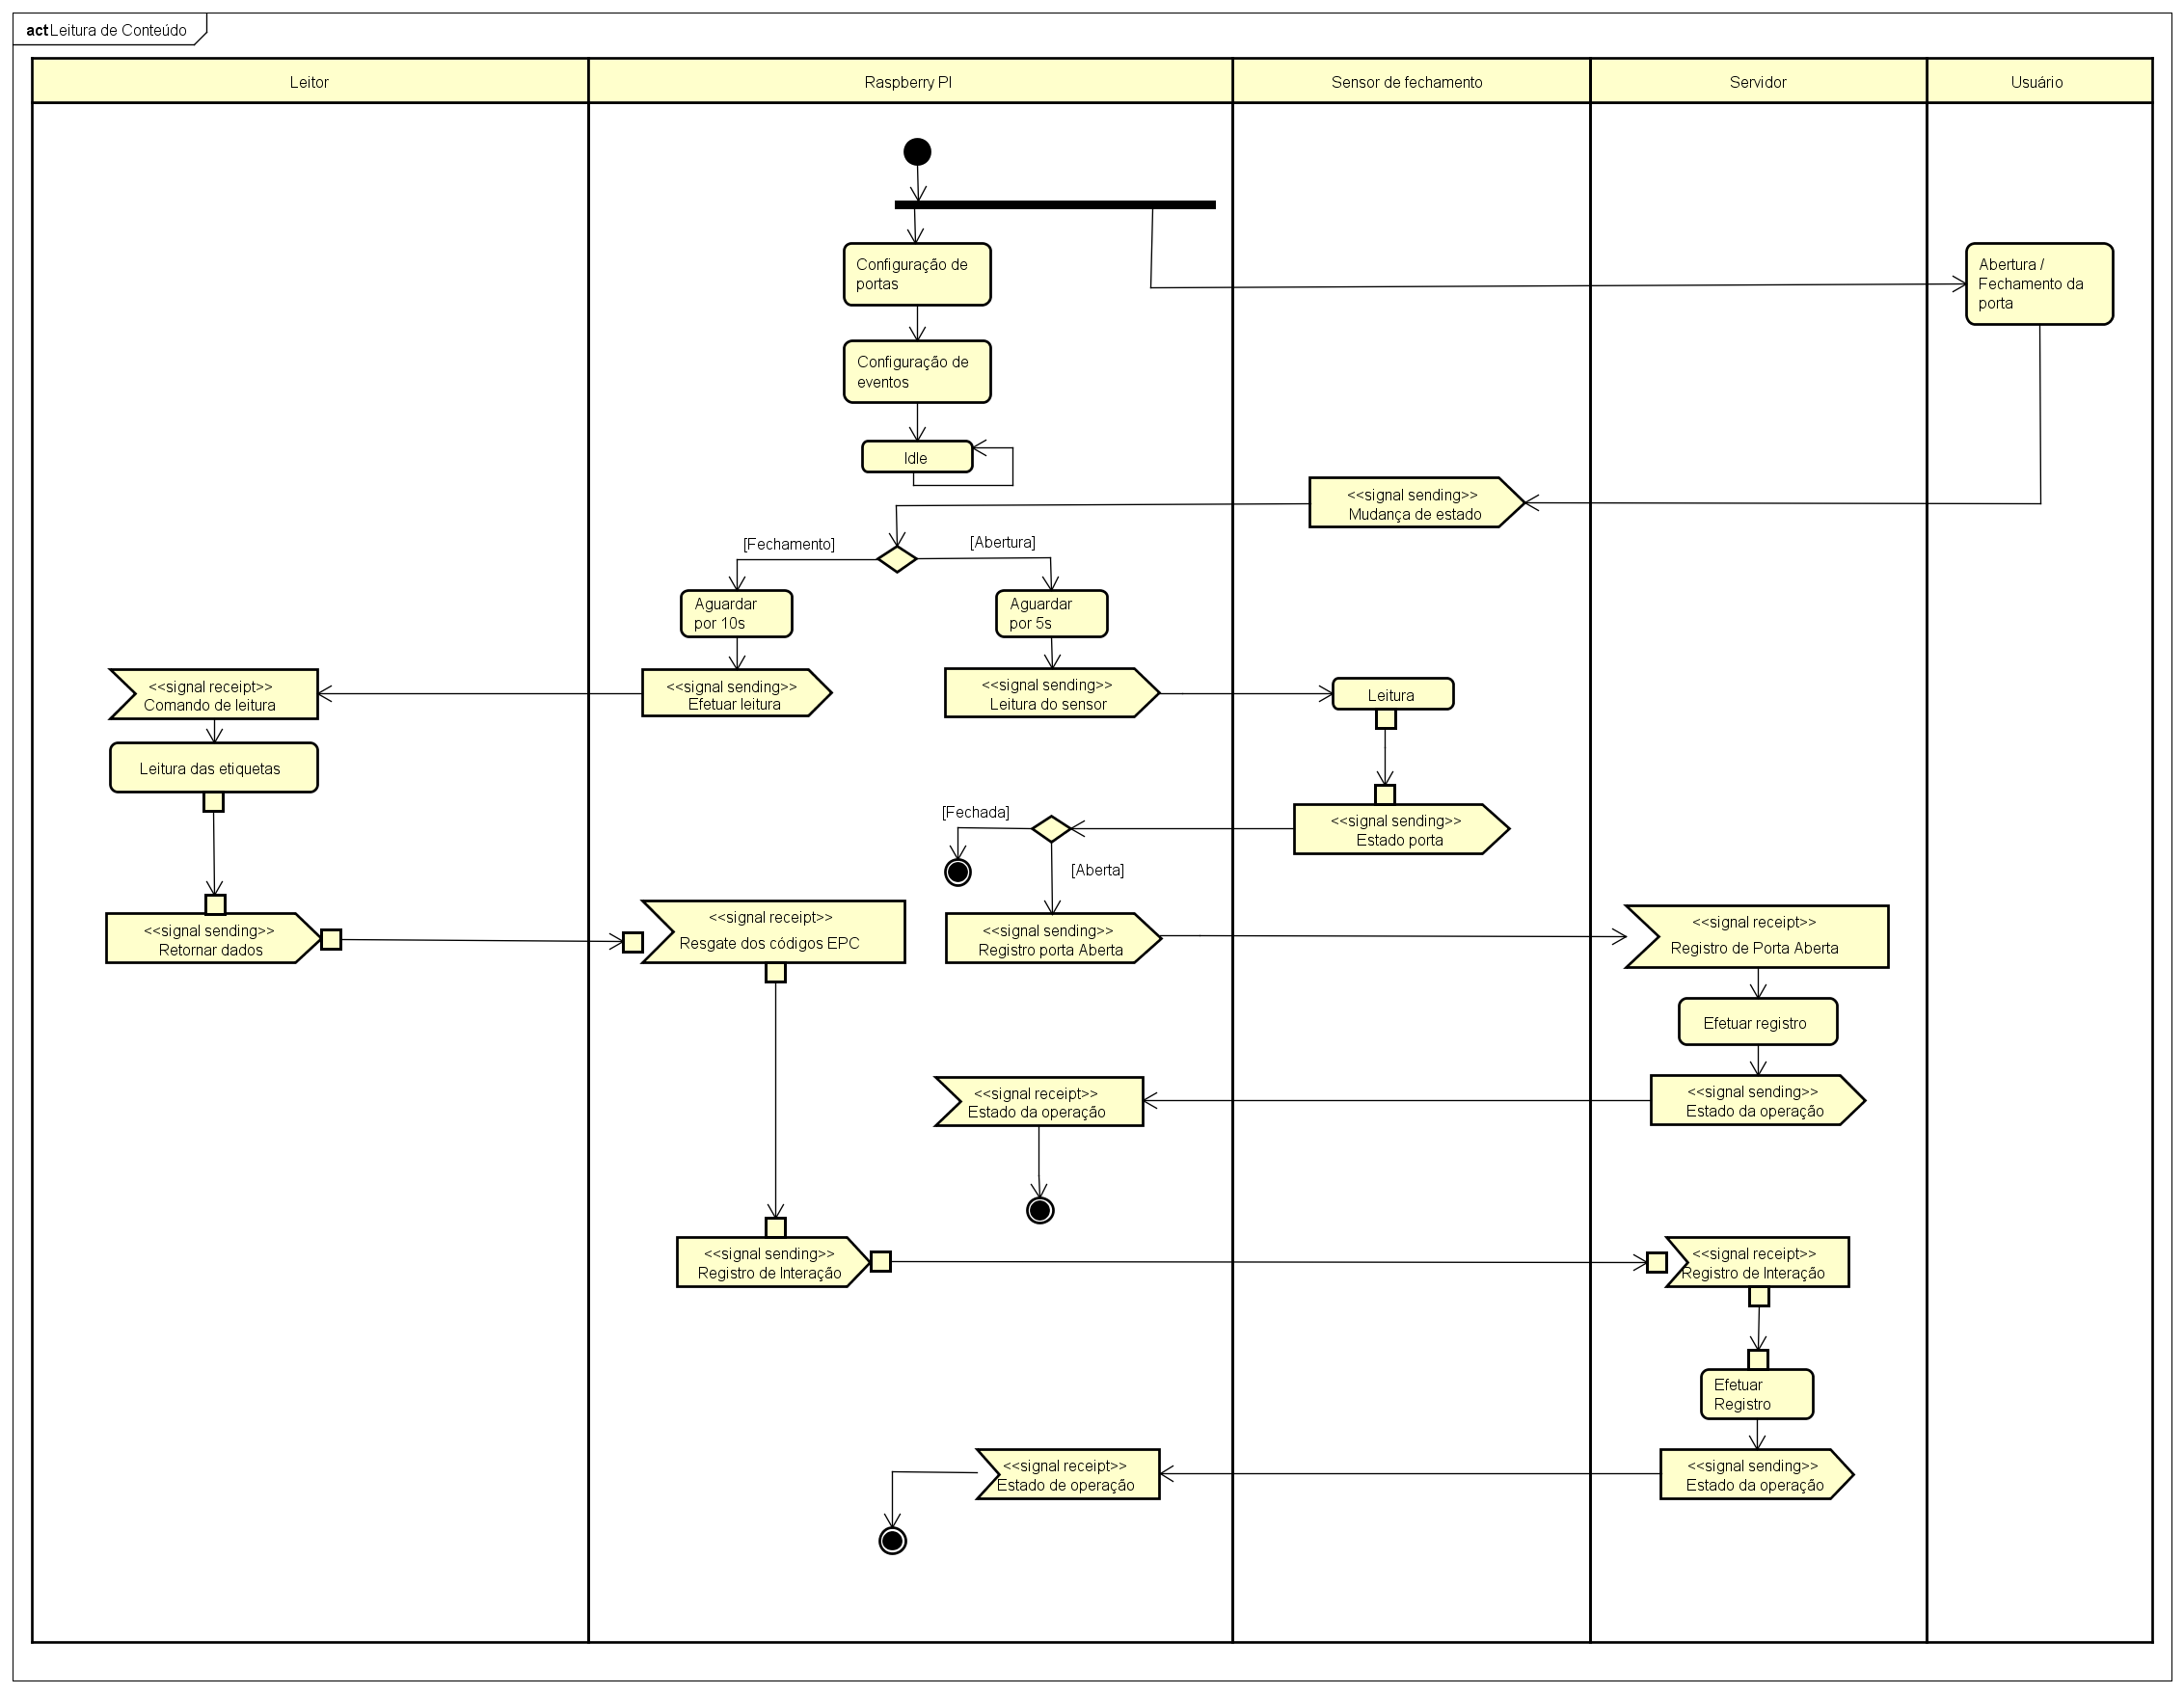
\includegraphics[width=\textwidth]{diagramas/diagr_leitura.png}
    
    \footnotesize{Fonte: Elaborado pelo Autor}
\end{figure}

%%%%%%%%%%%%%%%%%%%%%%%%%%%%%%%%%%%%%%%%%%%%%%%%%%%%%%%%%%%%%%%%%%%%%%%%%
\subsection{Listagem de conteúdo da geladeira}

Como uma continuação do processo anterior, o processo de listagem de produtos disponibiliza na interface o conjunto de produtos disponíveis. A Figura \ref{fig:cap5_diagr_lista_prod} demonstra o fluxo de atividades para este processo.

O gatilho para tal ação é dado na interface e esta enviará uma requisição da lista de produtos referentes à uma geladeira específica. Ao receber a solicitação, o servidor fará uma busca na base de interações pelo último registro gravado ao qual contém os códigos EPC lidos das etiquetas. Após isso, tendo o conjunto de códigos EPC, fará uma busca pelo produto correspondente a cada um. Assim, se terá uma lista de produtos e suas respectivas quantidades. Por fim, a lista de produtos, em formato JSON, é retornada à interface e apresentada ao usuário.

% Demonstrar fluxo de execução de listagem de produtos
\begin{figure}[htb]
    \caption{Listagem de conteúdo da geladeira}
    \label{fig:cap5_diagr_lista_prod}
    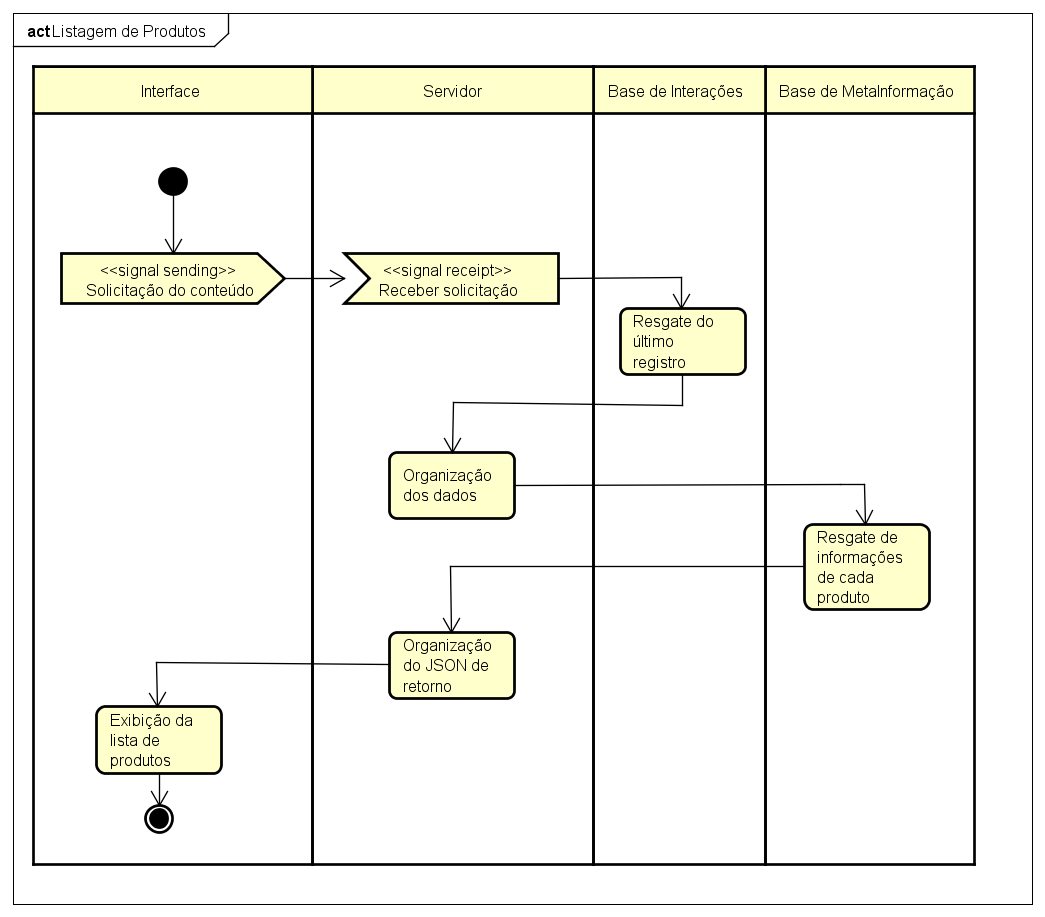
\includegraphics[width=\textwidth]{diagramas/diagr_lista_prod.png}
    
    \footnotesize{Fonte: Elaborado pelo Autor}
\end{figure}

\subsection{Geração de Recomendação de Produtos Novos} \label{ssec:geracao_rec_novo}

O processo de geração de recomendações, como já dito, é automaticamente inicializado pelo servidor, conforme Figura \ref{fig:cap5_diagr_geracao_rec}. Inicialmente, a matriz de frequência de interações de usuários com produtos é criada. Vale destacar, que um usuário se refere à uma geladeira. Em seguida, busca-se, na base de interações, todas as interações armazenadas. A partir das interações, na base de metainformação é feita a combinação entre códigos EPC e código de barras. A matriz de frequências é, então, preenchidas com os dados obtidos no processo anterior.

Como parte do cálculo da correlação de Pearson, a média de interações de cada usuário deve ser calculada. Logo após, é computada a similaridade entre os pares de usuários, indicados na Figura \ref{fig:cap5_diagr_geracao_rec} como $U1$ e $U2$, com a Equação \ref{eq:correlacao-pearson}.

Em posse das similaridades entre usuários, inicia-se o processo de recomendação para cada usuário ($U1$) cadastrado no sistema. Inicialmente, o conjunto de similaridades do usuário $U1$ com os demais é ordenado em ordem decrescente, ou seja, do usuário com maior similaridade ao menor. Em seguida, para cada usuário $U2$ na lista de similaridades é feita uma subtração de conjuntos de produtos aos quais $U2$ interagiu pelos que $U1$ o fez. Assim, tem-se um conjunto de produtos que $U1$ não conhece e que poderão ser sugeridos como novas opções de compra. 

O processo citado é repetido até que todos os usuários na lista de similares forneçam recomendações ou quando o número máximo de produtos recomendados for atingido. E, quando uma das duas possibilidades ocorrer, o conjunto de recomendações será salvo na base de recomendações e o o processo de recomendação se repetirá para o próximo usuário.

% Demonstrar fluxo de execução de geração de recomendação
\begin{figure}[H]
    \caption{Geração de Recomendações Novos} 
    \label{fig:cap5_diagr_geracao_rec}
    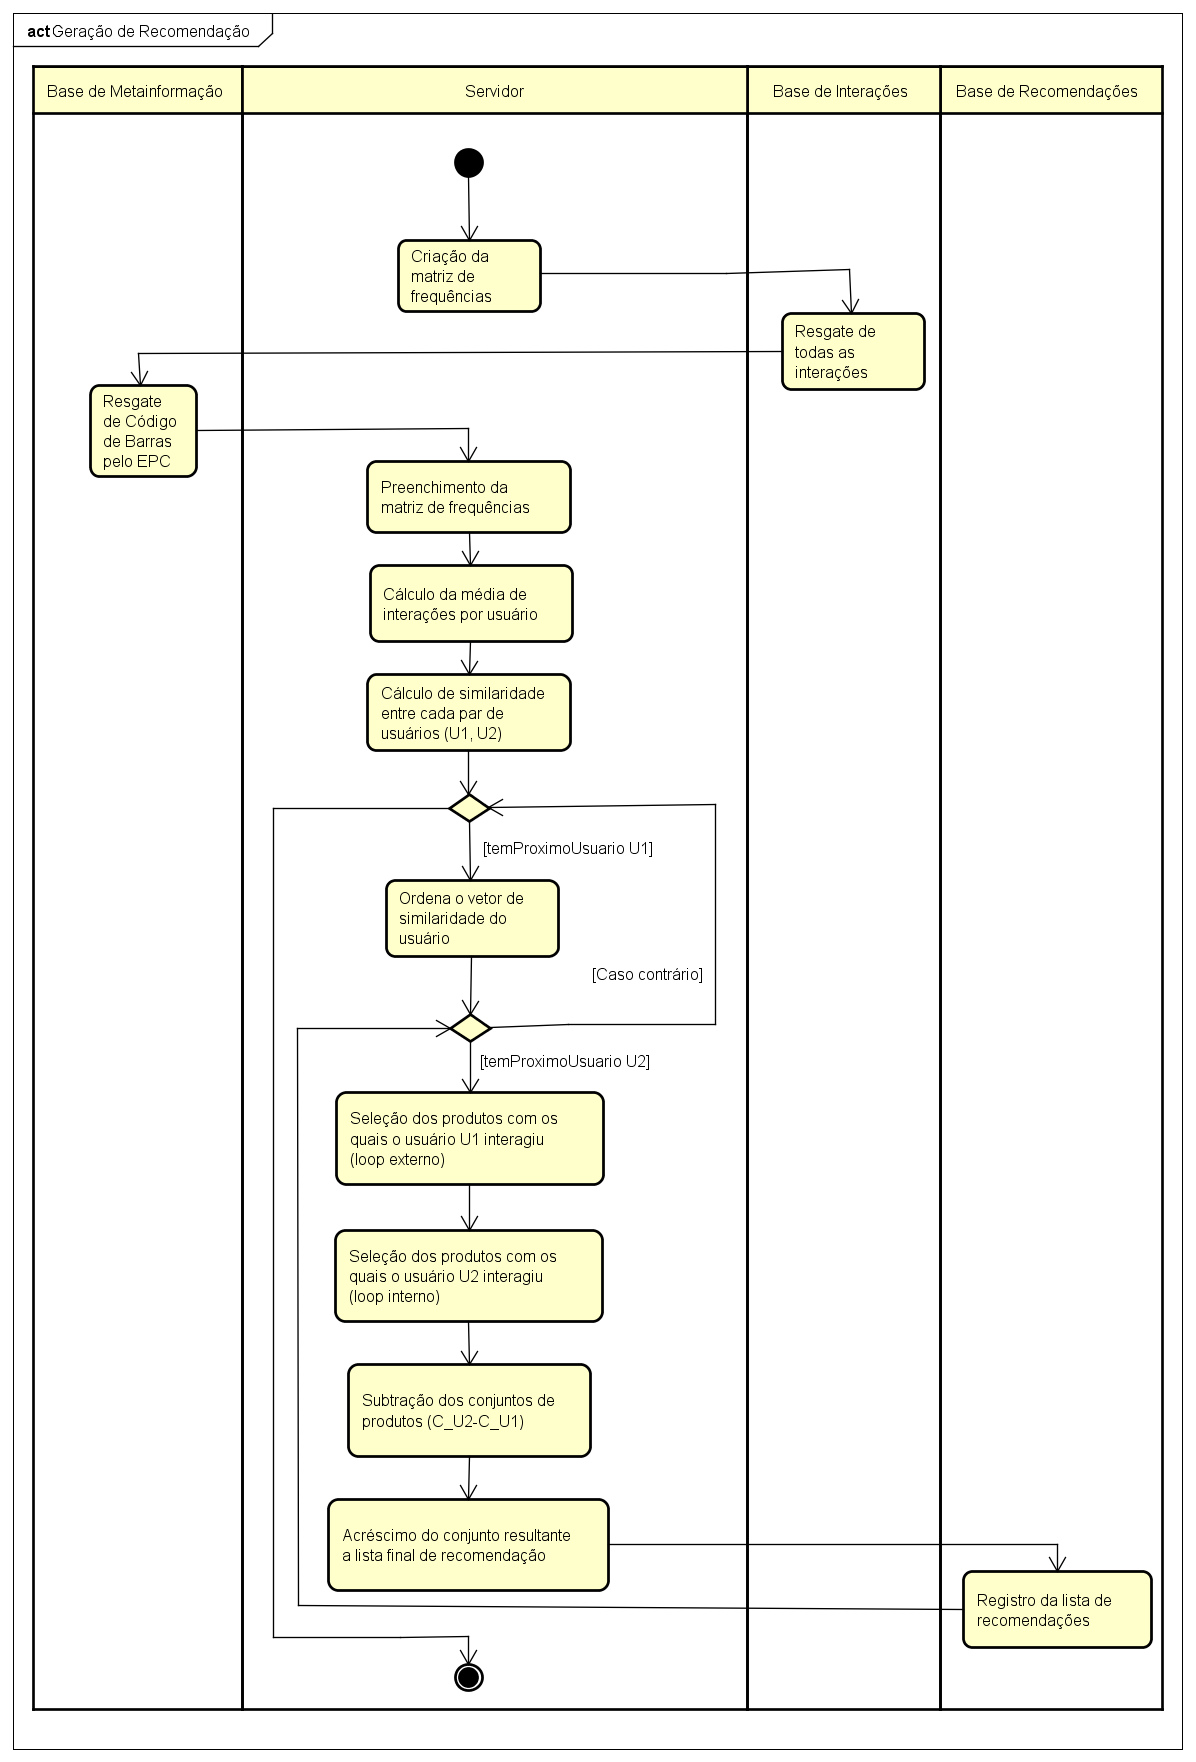
\includegraphics[width=\textwidth]{diagramas/diagr_geracao_rec.png}
    
    \footnotesize{Fonte: Elaborado pelo Autor}
\end{figure}

%%%%%%%%%%%%%%%%%%%%%%%%%%%%%%%%%%%%%%%%%%%%%%%%%%%%%%%%%%%%%%%%%%%%%%%%%
\subsection{Geração de Recomendação de Produtos Faltantes}

Da mesma forma que a seção anterior, o processo de recomendação é iniciado automaticamente pelo servidor, conforme Figura \ref{fig:cap5_rec_produto_faltante}. A partir disso, para que se recomende produtos, é necessário ter as listas de produtos disponíveis atualmente e de produtos requisitados. Para tanto, inicialmente, a base de interações é consultada para o resgate da última interação, tendo esta a indicação dos itens mais recentes. A partir da lista de códigos EPC extraídos da interação, é feita uma consulta à base de metainformação para que sejam obtidos os dados dos produtos.

O próximo passo é realizar o resgate, na base de estruturas auxiliares, das informações de configuração do usuário, às quais indicam os produtos essenciais. A partir da extração desse dado, é feita uma comparação de quantidade entre produtos disponíveis e essenciais. Caso o produto essencial esteja disponível na quantidade necessária, nada acontece. No entanto, caso o produto esteja disponível e em quantidade insuficiente, este é inserido na lista de recomendações tendo como quantidade sugerida a diferença entre o valor necessário e o existente. Caso o produto necessário não exista, sugere-se a quantidade total indicada nas configurações.

A seguir, para o conjunto de produtos recomendados, é feita uma verificação da disponibilidade desses produtos e na quantidade especificada. Assim, caso o esteja, uma indicação positiva será enviada. Caso contrário, o serviço do mercado fará uma busca por um produto similar e retornará tal item como alternativa. Por fim, pode haver casos em que nenhum item similar exista. Assim, apenas uma indicação negativa é retornada.

Com o conjunto de produtos indicados pelo mercado como disponíveis para compra, a lista final de recomendações é criada e inserida na base de recomendações.

\begin{figure}[H]
    \caption{Geração de Recomendação de Produtos Faltantes} 
    \label{fig:cap5_rec_produto_faltante}
    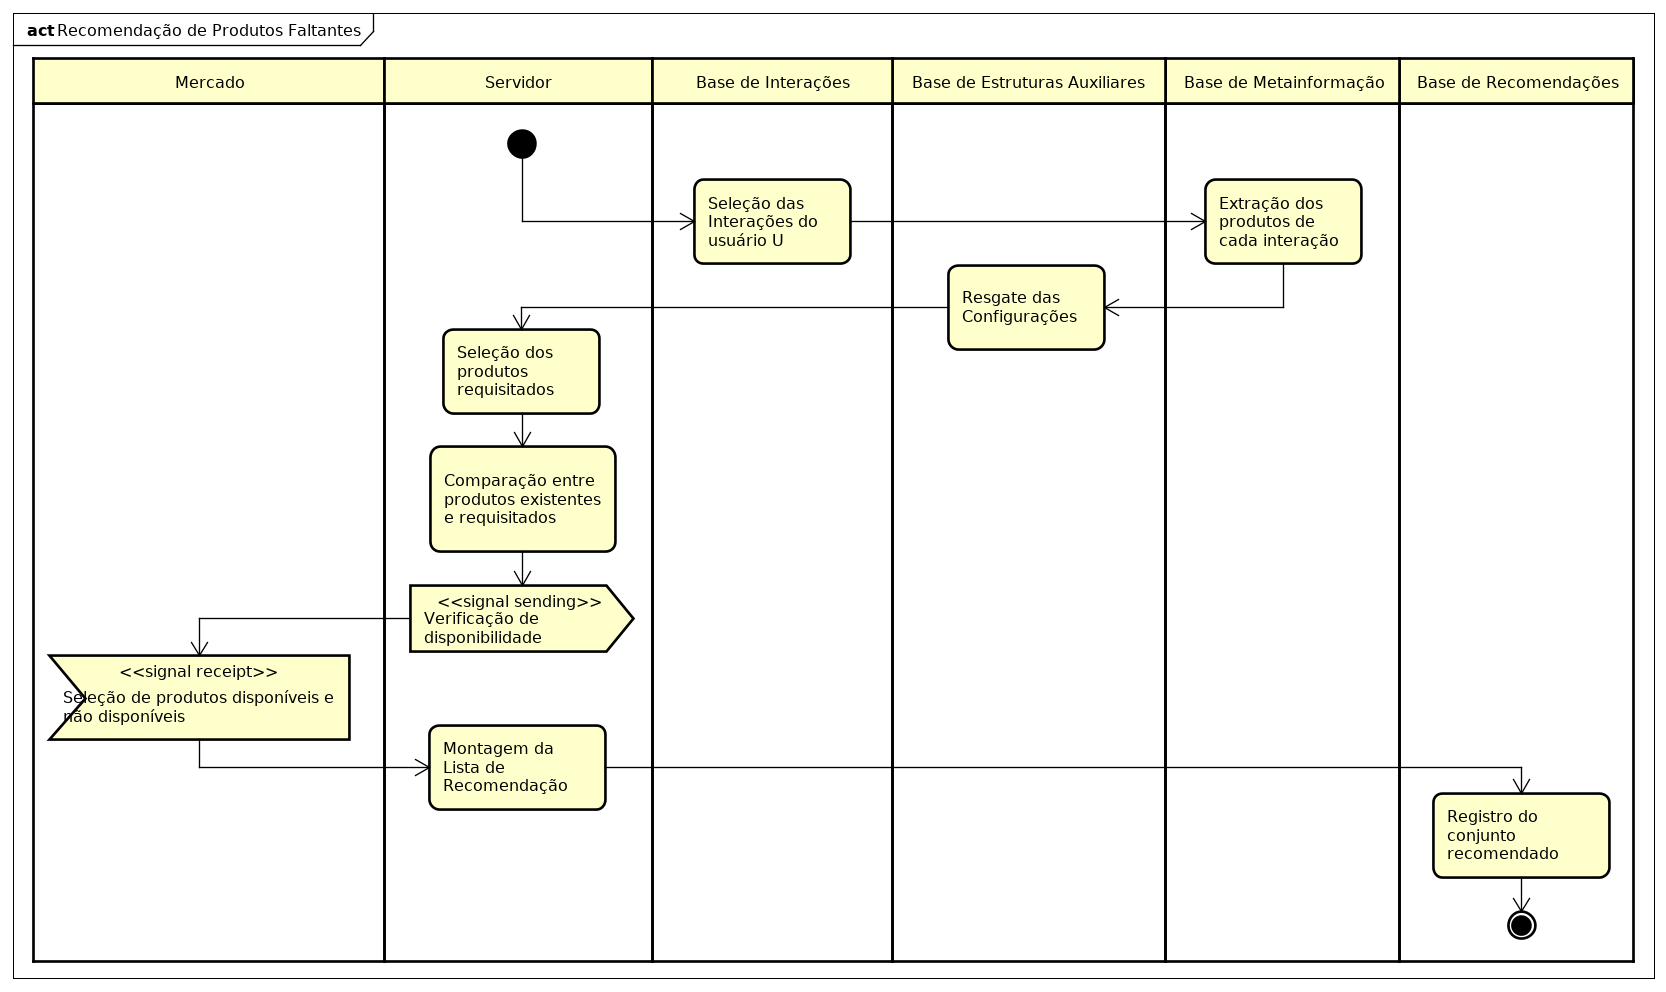
\includegraphics[width=\textwidth]{cap5_rec_produto_faltante}
    
    \footnotesize{Fonte: Elaborado pelo Autor}
\end{figure}

%%%%%%%%%%%%%%%%%%%%%%%%%%%%%%%%%%%%%%%%%%%%%%%%%%%%%%%%%%%%%%%%%%%%%%%%%
\subsection{Geração de Recomendação de Receitas por Conteúdo}

O processo de recomendação, conforme descrito na Seção X, decorre a partir da recomendação receitas que contenham alguns dos produtos disponíveis na geladeira. 

O processo é iniciado automaticamente no servidor e o primeiro passo se dá na seleção da última interação contendo os códigos EPC na respectiva base de dados.

A partir dos códigos EPC, obtém-se o conjunto de produtos correspondentes a ele, a partir da base de metainformação. Então, seleciona-se, na base de metainformação, as receitas que contenham pelo menos um dos produtos do conjunto e, a partir do número de correspondências entre produtos da lista selecionada e da receita, ordena-se o conjunto de receitas em ordem descendente, ou seja, receitas com maior número de correspondências primeiro. Por fim, o conjunto gerado é registrado na base de recomendações.

\begin{figure}[htb]
    \caption{Geração de Recomendação de Receitas por Conteúdo} 
    \label{fig:cap5_rec_receita_conteudo}
    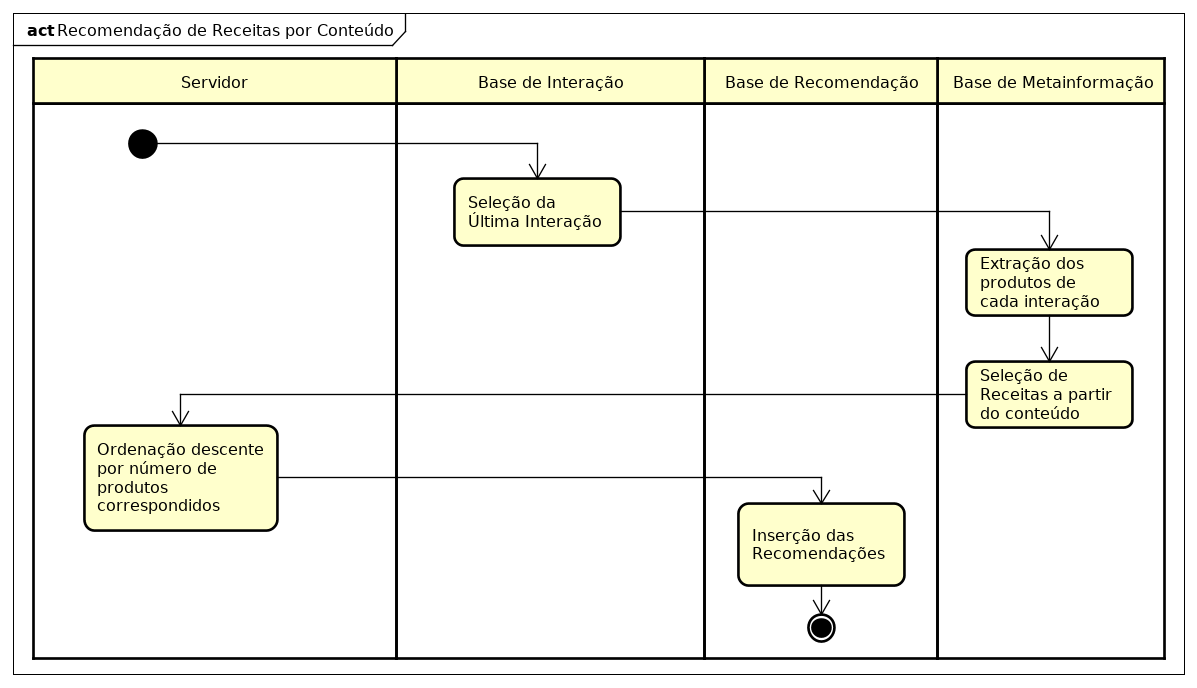
\includegraphics[width=\textwidth]{cap5_rec_receita_conteudo}
    
    \footnotesize{Fonte: Elaborado pelo Autor}
\end{figure}

%%%%%%%%%%%%%%%%%%%%%%%%%%%%%%%%%%%%%%%%%%%%%%%%%%%%%%%%%%%%%%%%%%%%%%%%%
\subsection{Geração de Recomendação de Receitas por Perfil}

A sugestão de receitas por perfil, conforme Figura \ref{fig:cap_diagr_receita_perfil} considera os produtos com os quais o usuário mais interagiu durante a escolha de quais receitas recomendar. Assim, como nos demais processos, inicia-se no servidor automaticamente. 

O primeiro passo consiste na seleção de todas as interações do usuário, na base de interações, seguida pela extração dos produtos de cada interação, na base de metainformação. A partir dai, a matriz de frequências é criada e preenchida a partir dos produtos obtidos e da quantidade de vezes em que aparecem nas interações. O próximo passo, portanto, é a ordenação descendente através da frequência. Os produtos com maior frequência serão, então, utilizados como base na seleção de receitas. Nessa implementação, limitou-se em cinco (5) o número de produtos utilizados.

Com a lista de produtos obtém-se o conjunto de receitas que contêm pelo menos um desses itens. O próximo passo consiste, então, em ordenar a lista em disposição descendente a partir do número de produtos na receita correpondidos na lista de produtos.

Por fim, o conjunto de receitas sugeridas é registrado na base de recomendações.

\begin{figure}[htb]
    \caption{Geração de Recomendação de Receitas por Perfil} 
    \label{fig:cap_diagr_receita_perfil}
    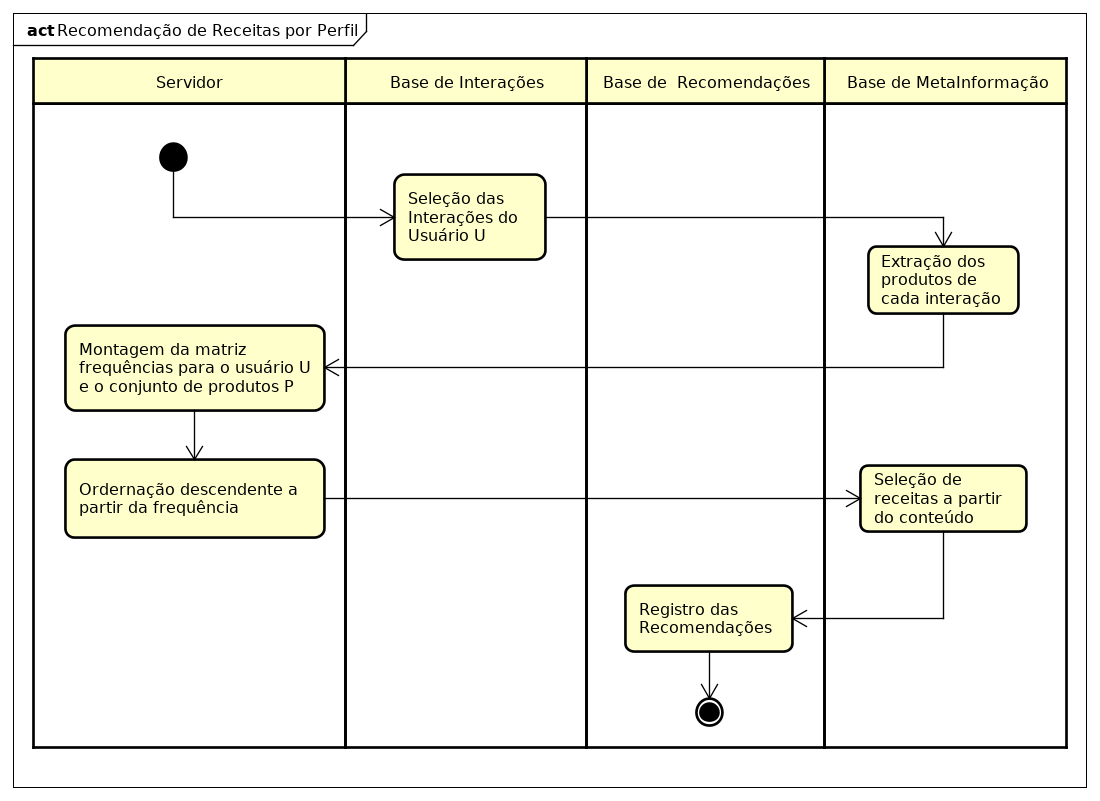
\includegraphics[width=\textwidth]{cap_diagr_receita_perfil}
    
    \footnotesize{Fonte: Elaborado pelo Autor}
\end{figure}


%%%%%%%%%%%%%%%%%%%%%%%%%%%%%%%%%%%%%%%%%%%%%%%%%%%%%%%%%%%%%%%%%%%%%%%%%
\subsection{Detecção e registro de porta aberta}

Considerando-se, inicialmente, que a geladeira se encontra fechada. Em uma dado momento, o usuário abre-a e insere e/ou retira produtos, no entanto, ao terminar, não fecha a porta.  No momento da abertura, o sistema da geladeira detecta a ação e inicia um período de espera. Ao final desse tempo, um registro correspondente ao estado da porta é feito na base de estruturas auxiliares.

Com relação à consulta de estado da porta. Apesar de seu respectivo diagrama não ser apresentado neste trabalho, o fluxo é muito semelhante aos relacionados à consulta de listagem de produtos. Assim, quando a interface requerer o estado atual no servidor, receberá o último registro feito. A partir dele, caso indique estado aberto, uma notificação é emitida na interface.

\begin{figure}[htb]
    \caption{Detecção de porta aberta}
    \label{fig:cap5_diagr_porta_aberta}
    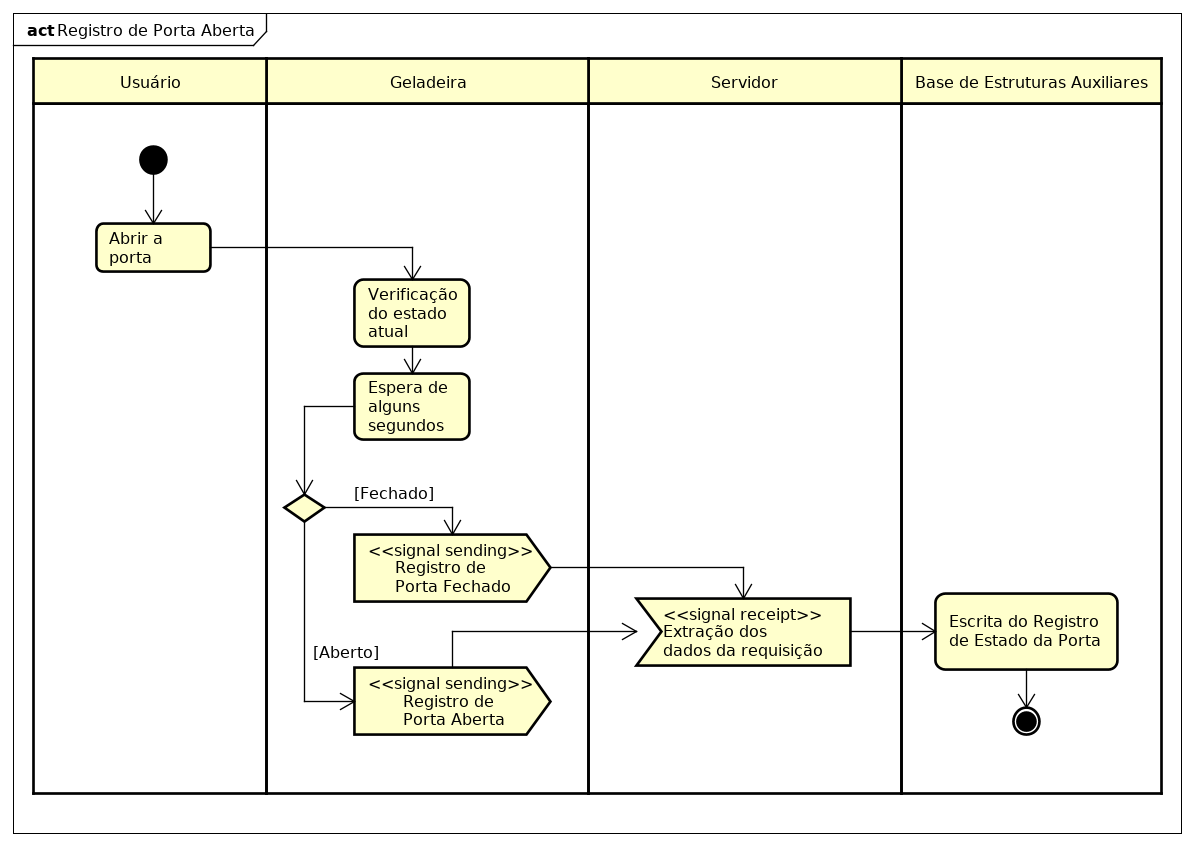
\includegraphics[width=\textwidth]{cap5_diagr_porta_aberta}
    
    \footnotesize{Fonte: Elaborado pelo Autor}
\end{figure}

\subsection{Listagem de Recomendações} \label{ssec:listagem_rec}

O processo de listagem de recomendações é engatilhado na interface de usuário. Desse modo, a interface envia uma requisição ao servidor solicitação um conjunto de recomendações para um determinado usuário, conforme Figura \ref{fig:cap5_diagr_lista_rec}.  Ao receber a solicitação, o servidor, faz uma busca na base de recomendações pelos produtos recomendados. Em seguida, os dados são organizados e o conjunto de recomendação é enviado à interface.

% Demonstrar fluxo de execução de listagem de recomendação
\begin{figure}[htb]
    \caption{Listagem de Recomendações}
    \label{fig:cap5_diagr_lista_rec}
    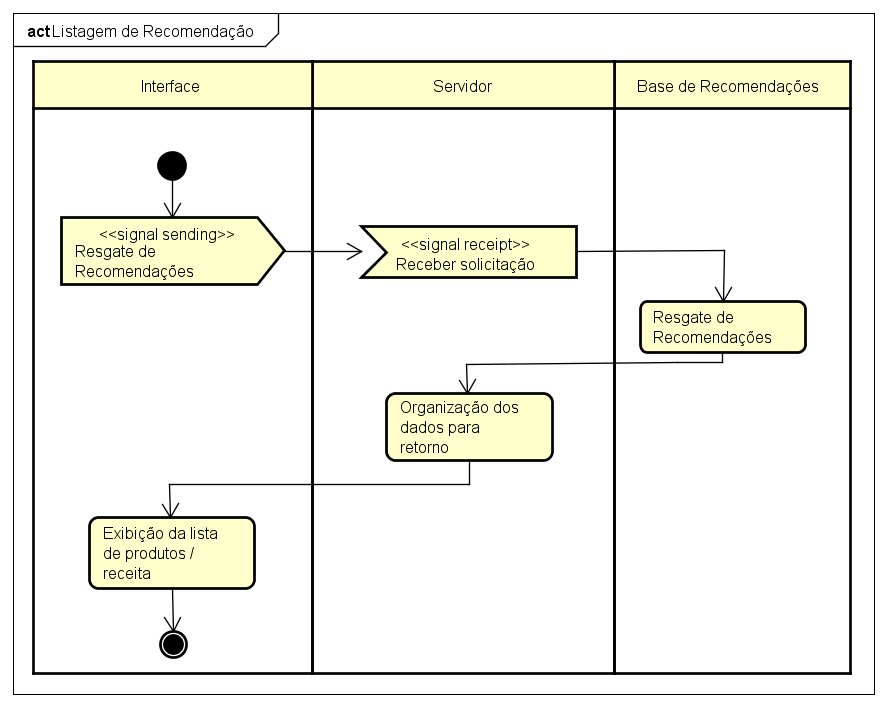
\includegraphics[width=\textwidth]{diagramas/diagr_list_rec.png}
    
    \footnotesize{Fonte: Elaborado pelo Autor}
\end{figure}

% Demonstrar fluxo de execução de listagem de produtos

\section{Cenário de Aplicação}

A avaliação do modelo dar-se-á a partir do ambiente ilustrado na Figura \ref{fig:cap5_ambiente-cenario}. O ambiente consiste na demonstração de uma sequência de ações, começando pela interação do usuário, com o objetivo de observar o efeito no protótipo implementado.

\begin{figure}[htb]
    \caption{Ambiente do cenário}
    \label{fig:cap5_ambiente-cenario}
    \includegraphics[width=\textwidth]{figuras/cap5_cenario.png}
    
    \footnotesize{Fonte: Elaborado pelo Autor}
\end{figure}

Em relação, as bases de dados, essas foram preenchidas antes da avaliação do sistema. 
% Descrição dos dados de produtos
Primeiramente, para a base de metainformação foram alocadas informações de quarenta (40) produtos, extraídas dos produtos originais em um supermercado na cidade de Araranguá. Excetua-se apenas o endereço URL da imagem de cada produto ao qual foi obtido web-sites de supermercados. 
% Descrição de dados de receitas
Já em relação às receitas, utilizou-se de dez (10) receitas obtidas a partir de sites de culinária. Tanto informações  de produtos quanto receitas foram formatadas conforme a Seção \ref{sssec:metainfo}.

% Descrição da quantidade de usuários
Quanto à identificação das geladeira e, por consequência, dos usuários, não criou-se uma base específica para eles, apenas atribuiu-se um identificador utilizado em cada registro específico a um determinado usuário. Como definiu-se dez (10) geladeiras, foram definidos os valores de um (1) a dez (10) para diferenciação de cada uma.

% Descrição da quantidade de interações por usuários.
Para cada geladeira, foram criadas, de maneira aleatória, interações, cada qual com um conjunto de códigos EPCs representandos os produtos. Assim, definiu-se que o número de interações seria maior ou igual a cinco (5) e menor ou igual a 25. Além disso, para cada interação o número mínimo de itens registrados seria de três (3) e, no máximo, 10.

% Configurações de produtos
Em relação às configurações, descritas na Seção \ref{sssec:base_est-aux}, todos as geladeiras apresentaram parâmetros idênticos excetuando-se as listas de produtos essenciais e suas respectivas quantidades mínimas. Assim, quais produtos e quais quantidades foram definidas randomicamente. Quanto à quantidade de produtos requisitados, estabeleceu-se o número de cinco (5) produtos e, em relação à quantidade, definiu-se um valor randômico entre um (1) e vinte (20).

% Quais os produtos que têm RFID que serão usados na geladeira
Como forma de teste do protótipo da estrutura física da geladeira, três produtos receberam etiquetas com o respectivo código EPC. Sendo eles...
% TODO:  Especificar os produtos


%%%%%%%%%%%%%%%%%%%%%%%%%%%%%%%%%%%%%%%%%%%%%%%%%%%%%%%%%%%%%%%%%%%%%%%%%%%%%%%%%%%%%%%%%%%%%%%%%%%%%%%%%%%%%%%%%%%%%%%%%%%%%%%%%%%%%%%%%%%%%%%%%%%%%%%%%%%%%%%%%%%%%%%%%%%%%%%%%%%%%%%%%%%%%%%%%%%%%%%%%%%%%%%%%%%%%%%%%%%%%%%%%%%%%%%%%%%%%%%%%%%%%%%%%%%%%%%%%%%%%%%
\section{Avaliação do Protótipo}

\subsection{Leitura do conteúdo}
 Inicialmente a geladeira está vazia.
 Ao colocar dois produtos, sendo eles, o ``Margarina com Sal Qualy'' e ``Creme de Leite Tirol'', respectivamente, depois de alguns minutos os seguintes códigos EPC são lidos.
 
 \begin{itemize} \parskip -3pt
     \item 8665580279609348107299713701
     \item 8665580277303506451141610373
 \end{itemize}
 
 Os dados são, então, enviados ao serviço de registro de interação e o registro, da Figura \ref{fig:cap5_registro_interacao}, é gravado na base de interações. 
 
 \begin{figure}[htb]
     \caption{Registro de interação dos produtos}
     \label{fig:cap5_registro_interacao}
     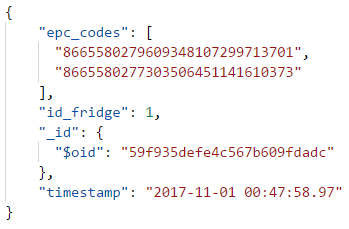
\includegraphics[width=0.5\textwidth]{cap5_registro_interacao}
     
     \footnotesize{Fonte: Elaborado pelo Autor}
 \end{figure}
 
 %%%%%%%% JSON DO REGISTRO  %%%%%%%%
\subsection{Listagem de conteúdo da geladeira}
 
Continuando o fluxo da seção anterior, ao tentar ler o conteúdo da geladeira logo após o fechamento da porta, a listagem da interface continua sendo vazio. Alguns segundos depois, a listagem é atualizada e o conteúdo exibido é mostrado na Figura \ref{fig:cap5_listagem_atual}.


 %%%%%%%%%%%%%%%%%%%%%   FIGURA DA LISTAGEM APÓS A INTERAÇÃO %%%%%%%%%%%%%%%%%%%%%%%%%%%%%%%%%%%
\begin{figure}[htb]
    \caption{Listagem de produtos na Interface}
    \label{fig:cap5_listagem_atual}
    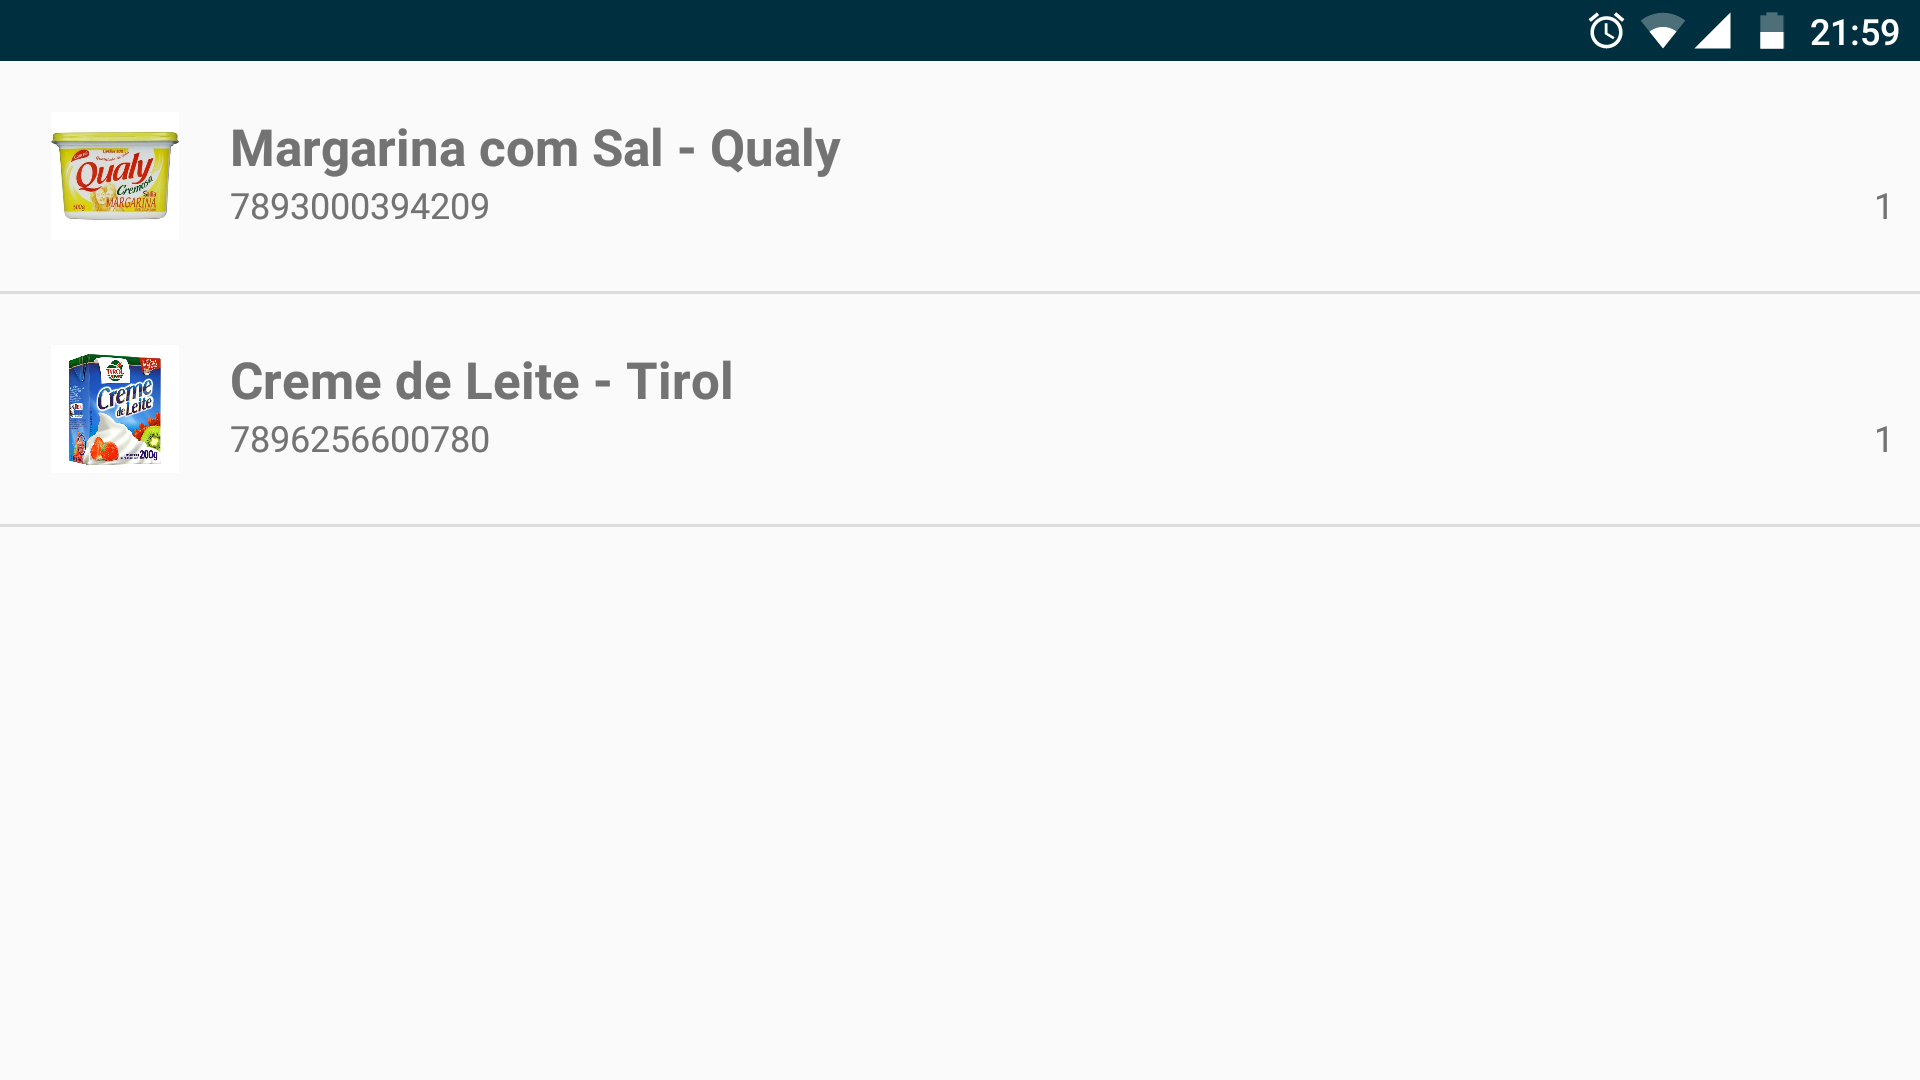
\includegraphics[width=0.8\textwidth]{cap5_listagem_atual}
    
    \footnotesize{Fonte: Elaborado pelo Autor}
\end{figure}
 
Dessa forma, afirma-se que a listagem de produtos está operando de acordo com o esperado, já que a lista é alterada após a interação. No entanto, o fator temporal entre a interação e a exibição é compreensível. Assim, o intervalo de tempo decorre do aguardo, na geladeira, até a realização da leitura. Isso é necessário para garantir que teve tempo hábil para coletar ou inserir todos os produtos que deseja-se.


%%%%%%%%%%%%%%%%%%%%%%%%%%%%%%%%%%%%%%%%%%%%%%%%%%%%%%%%%%%%%%%%%%%%%%%%%%%%%%%%%%%%%%%%%%%%%%
\subsection{Geração de Recomendações de Produtos Novos}

Deseja-se gerar recomendações para o Usuário 1. Para tanto, seguiu-se o fluxo da Seção \ref{ssec:geracao_rec_novo}. Os passos foram executados até o cálculo de similaridade entre usuários sobre a matriz de frequências de interações e obteve-se o usuário mais semelhante. Tal indivíduo é identificado como Usuário 10 e o grau de similaridade entre este o Usuário 1 foi de 0,15 e a média de interações foi de 2,05 o primeiro e 2,12 para o décimo.

%inicia-se com a criação da matriz de frequências seguida pelo resgate das interações e, a partir dessas, dos códigos de barras e, por fim o preenchimento da matriz, conforme Figura \ref{fig:cap5_diagr_geracao_rec}.

Como forma de verificação, tem-se as linhas da matriz de frequência, conforme Tabela \ref{tab:cap5_matriz_sim}, referentes aos usuários.


%%%%%%%%%%%%%%%%%%  MATRIZ  %%%%%%%%%%%%%%%%%%%%%%
\begin{table}[htb]
\caption{Matriz de similaridade}
\label{tab:cap5_matriz_sim}
\begin{tabular}{C{0.8cm}c}
\toprule
%\rotatebox[origin=c]{270}{B}\\
\textbf{U1} & 0 2  2  6  2  3  6  0  2  4  2  5  2  1  1  2  1  8  5  6  5  1  2  3  3  5  5  3  1  0  0  0  0  0  0 \\ \midrule
\textbf{U10} & 2  2  7  3  3  3  4  3  0  0  2  4  0  0  4  0  2  9  6  0  2  0  0  5  4  0  2  3  1  2  4  7  5  2  3 \\ \bottomrule
\end{tabular}
\end{table}        

Executando o cálculo da correlação de Pearson, descrita na Equação \ref{eq:correlacao-pearson}.

%%%%%%%%%%%%%%%%%%  EQUAÇÃO COM VALORES SUBSTITUÍDOS  %%%%%%%%%%%%%%%%%%%%%%%%%%%%%%
\begin{equation}
sim=\dfrac{\left[
\splitdfrac{
(0-2,05)(2-2,12)+
(2-2,05)(2-2,12)+
}
{\splitdfrac{
(2-2,05)(7-2,12)+
(6-2,05)(3-2,12)+
}{
(2-2,05)(3-2,12)+...}}\right]}
{
\left[
\splitdfrac{
\sqrt{\splitdfrac{(0-2,05)^2+
(2-2,05)^2+
(2-2,05)^2+
}{
(6-2,05)^2+
(2-2,05)^2+...}}
}{
\times\sqrt{\splitdfrac{(2-2,12)^2+
(2-2,12)^2+}{\splitdfrac{
(7-2,12)^2+
(3-2,12)^2+
}{
(3-2,12)^2+...}}}
}\right]
}
\nonumber
\end{equation}

\begin{equation}
sim = 0,15 \nonumber
\end{equation}

Assim, demonstra-se que o cálculo de similaridade está correto.

Percebe-se que o número de produtos com os quais o Usuário 1 não apresentou nenhuma interação, ou seja, as posições na linha do usuário mencionado preenchidas com zero (0), é oito (8). Assim, espera-se que pelos menos esses produtos sejam recomendados. 
No entanto, um número maior de itens podem ser sugeridos. Isso ocorrerá quando a quantidade obtida de recomendações através do usuário, com maior similaridade, for insuficiente. Assim, recomendações de outros usuários, com graus de semelhança menores, serão consideradas.

Obteve-se, a partir da consulta à base de recomendações, a seguinte lista de itens:

\begin{itemize} \parskip -3pt
    \item 7892840800000 - Refrigerante Pepsi
    \item 789034630442 - Creme de Leite Parmalat
    \item 7894900093056 - Iogurte Danone
    \item 7896648699453 - Leite Integral Langaru
    \item 7894904326044 - Pizza Calabresa Seara
    \item 7891991010481 - Cerveja Budweiser
    \item 7896256603422 - Leite Desnatado Tirol
    \item 7896256602050 - Iogurte de Morango Tirol
    \item 7891025101376 - Iogurte Danone
    \item 7896034680010 - Leite Condensado Parmalat
    \item 7891515490430 - Lasanha Calabresa Perdigão
\end{itemize}

 %%%%%%%%%%%%%%%%%%%%%   FIGURA DA LISTAGEM DE RECOMENDAÇÕES DE PRODUTOS NOVOS %%%%%%%%%%%%%%%%%%%%%%%%%%%%%%%%%%%

Os primeiros oito produtos da lista são aqueles que o Usuário 1 não interagiu, mas que o Usuário 10 o fez, na mesma sequência mostrada na Tabela \ref{tab:cap5_matriz_sim}. Já os demais três itens foram sugeridos com base em outros usuários com menor similaridade.
Além disso, vale ressaltar que o JSON gerado pelo sistema não foi inserido diretamente neste trabalho, pois ocuparia algumas páginas sem a devida necessidade.

\subsection{Geração de Recomendações de Produtos Faltantes}

Nessa seção, busca-se avaliar a recomendação da reposição de produtos aos quais o Usuário 2 julga serem essenciais. Para tanto, considera-se o fluxo de execução demonstrado na Seção X e o conjunto de produtos contidos atualmente e suas respectivas quantidades :

%%%%%%%%%%%%%%% Lista de um conjunto de produtos atuais %%%%%%%%%%%%%%%
\begin{itemize} \parskip -3pt
    \item Mortadela Perdigão, 5 UN
    \item Pizza Calabresa Sadia, 4 UN
    \item Iogurte de Morango Activia, 5 UN
\end{itemize}

E o conjunto de produtos ditos essenciais:

%%%%%%%%%%%%%%% Lista de um conjunto de produtos essenciais %%%%%%%%%%%%%%%
\begin{itemize} \parskip -3pt
    \item Mortadela Perdigão, 8 UN
    \item Pizza Calabresa Sadia, 6 UN
    \item Iogurte de Morango Activia, 5 UN
    \item Linguiça de Pernil, 15 UN
    \item Leite integral Aurora, 8 UN
\end{itemize}


Percebe-se que alguns produtos estão ausentes e, outros, em falta como, por exemplo, o produto Pizza está em quantidade insuficiente e o produto Leite está ausente. Assim, a recomendação deve conter tais produtos além de outros não citados.

Seguindo o fluxo da Seção \ref{ssec:listagem_rec}, tem-se como listagem de sugestões na interface como é mostrado.

\begin{figure}[htb]
    \caption{Listagem de Recomendações por falta}
    \label{fig:cap5_rec_faltante}
    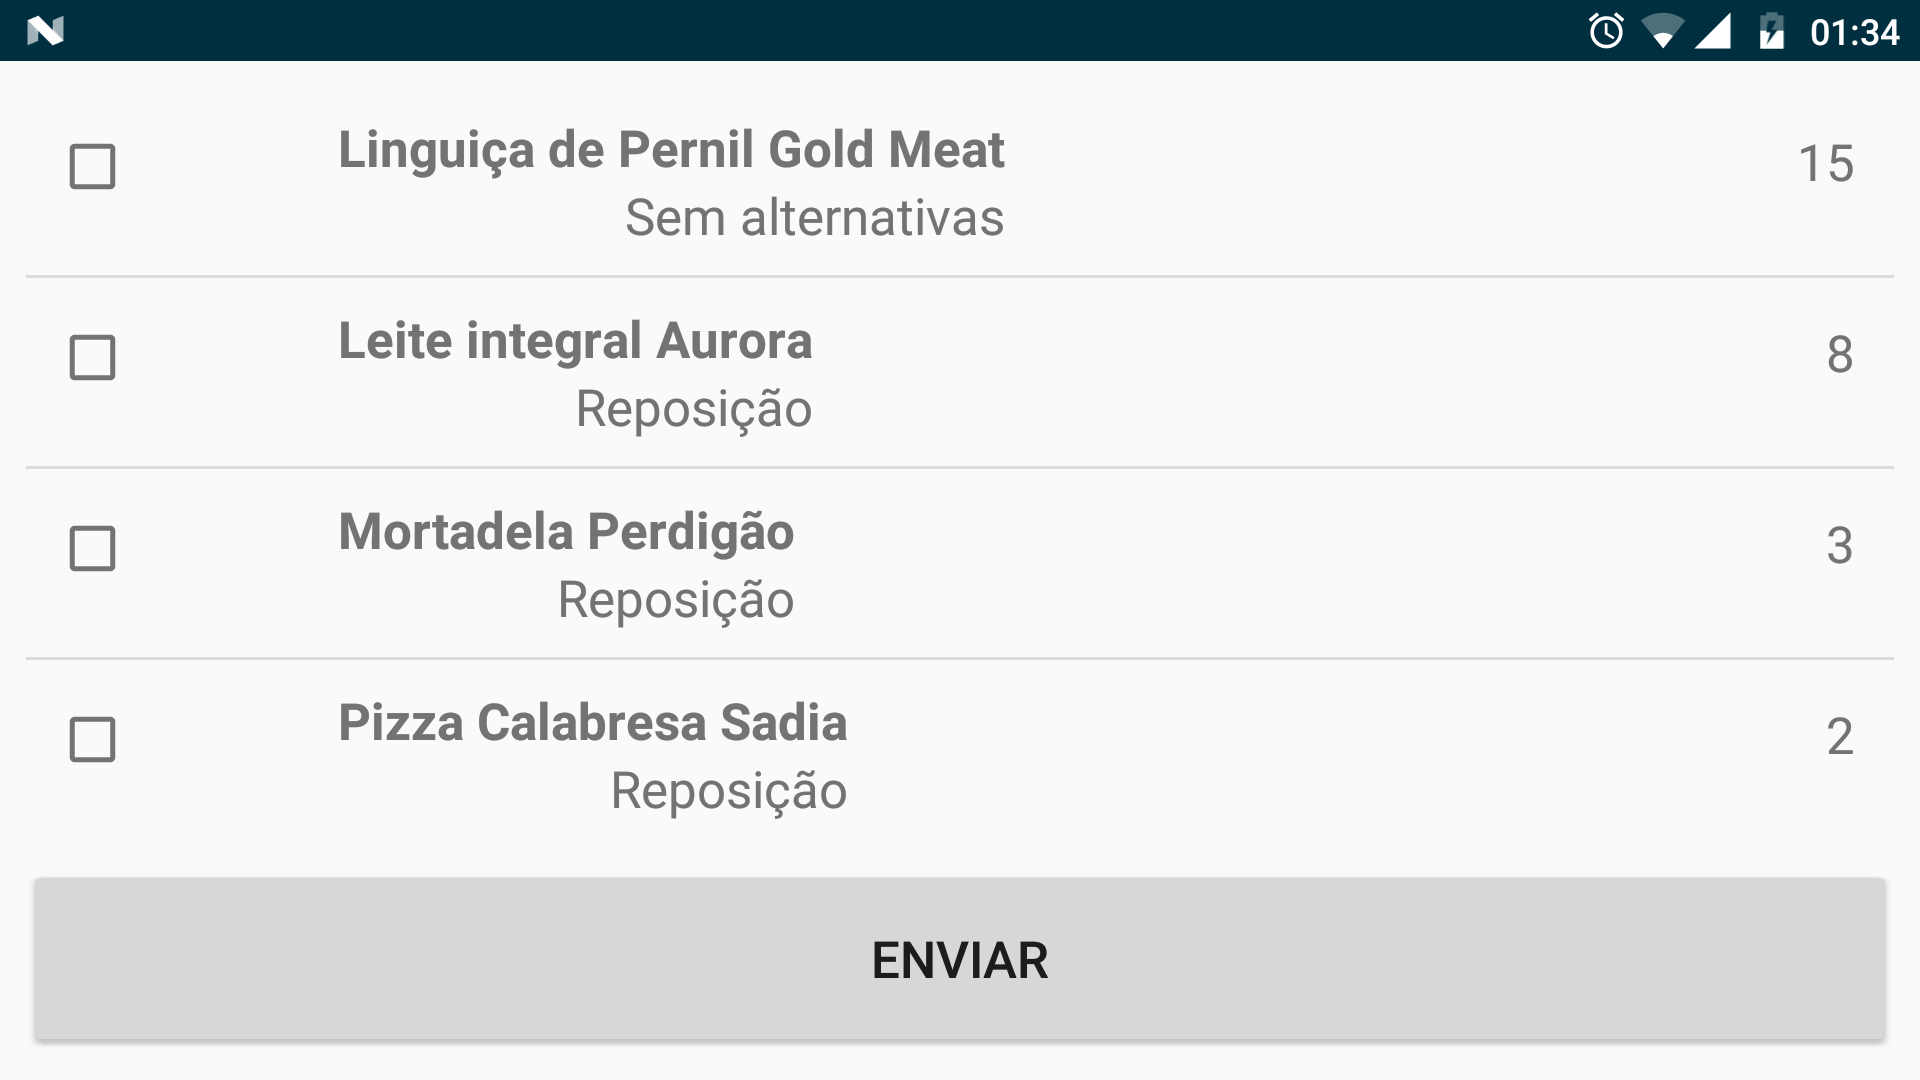
\includegraphics[width=0.8\textwidth]{cap5_rec_faltante}
    
    \footnotesize{Fonte: Elaborado pelo Autor}
\end{figure}

%%%%%%%%%%%%%%% Lista de um conjunto de produtos recomendados %%%%%%%%%%%%%%%

Percebe-se que há diferenciação entre os produtos, sendo de ``Reposição'' e ``Sem Alternativas''. A reposição trata da recolocação de produtos essenciais. O ``Sem alternativas'', indica que não foi possível encontrar no mercado, o produto esperado nem um similar a ele. Há, além disso, outras duas formas de recomendação de compras: ``Novo'', referente recomendação de produtos novos, como descrito anteriormente, além de ``Similar'' que indica a reposição de produtos essenciais que não estavam disponíveis no mercado, mas que foram substituídos por produtos idênticos.

\subsection{Geração de Recomendações de Receitas a partir de Conteúdo}

A recomendação de receitas por conteúdo, como descrito na seção respectiva no Capítulo 4, busca disponibilizar um conjunto de receitas ao usuário, de acordo com os itens que este possui em sua geladeira. 

Considera-se que, inicialmente, os seguintes produtos estejam disponíveis, e suas respectivas quantidades:

\begin{itemize} \parskip -3pt
    \item Leite Integral, com 2 UN
    \item Leite Condensado Parmalat com 3 UN 
    \item Queijo Mussarela Sadia, com 5 UN.
\end{itemize}

O processo de recomendação avaliará os produtos do ponto de vista de suas características, ou seja, terá um enfoque nos tipos de produtos e não em produtos de determinadas marcas.

O processo de recomendação analisa quais receitas satisfazem o requisito especificado e retornará um conjunto de itens para sugestão.

Os itens sugeridos como recomendações são mostrados na Figura \ref{fig:cap5_rec_recipe_content}.

%%%%%%%%%%%%%%%%%%    FIGURA X (Lista de receitas de recomendação)    %%%%%%%%%%%%%%%%%%%%%%%%%%%%%
\begin{figure}[htb]
\caption{Resultado da recomendação de receitas}
\label{fig:cap5_rec_recipe_content}
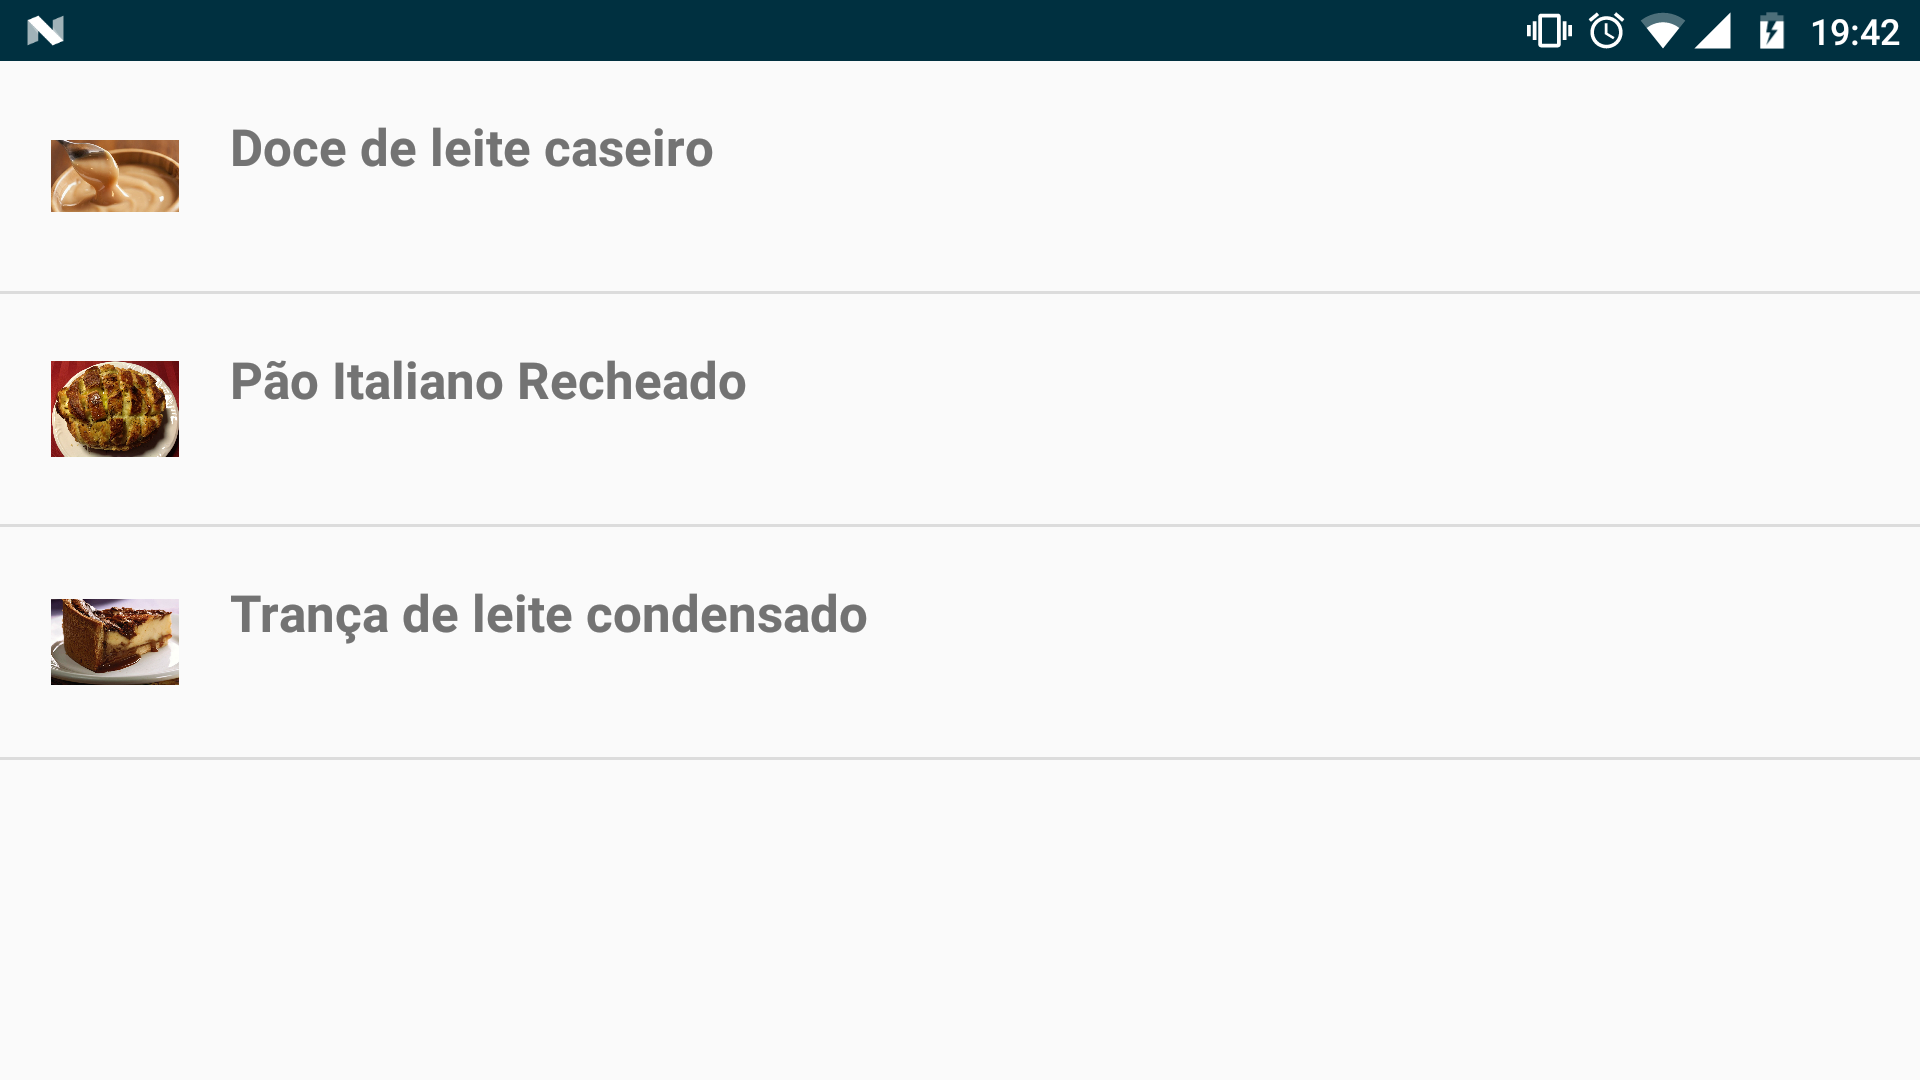
\includegraphics[width=0.8\textwidth]{cap5_rec_recipe_content}

\footnotesize{Fonte: Autor}
\end{figure}

Como resultado da recomendação, tem-se três receitas sugeridas dentre as cinco utilizadas nesse cenário, ou seja, duas receitas não incluíam nenhum dos produtos contidos na geladeira. A primeira receita na lista conta com o Leite, a segunda com o Queijo Mussarela e a terceira com Leite e Leite Condensado.

\subsection{Geração de Recomendações de Receitas por perfil}

Como descrito na seção \ref{sssec:proc_ger_rec}, a sugestão de receitas por perfil buscará receitas que contenham alguns dos itens com os quais o usuário mais interagiu. Para tanto, uma matriz de frequência de interações é montada.  Com base nas frequências de interações do usuário em questão, uma lista é criada a partir das classes de produto.

Considerando que limitou-se o total de produtos para geração de recomendação em cinco (5) e que estes são:

\begin{itemize} \parskip -3pt
    \item Margarina com Sal Qualy, com 9 interações
    \item Refrigerante de Guaraná Fanta, com 9 interações
    \item Linguiça de Pernil Gold Meat, com 8 interações
    \item Iogurte Danone, com 7 interações
    \item Queijo Mussarela Sulfrios, com 7 interações
\end{itemize}

Com base em tal conjunto, o processo de recomendação fez uma busca na base de interações pela receitas que contivessem tais categorias de produtos. A partir disso, o conjunto de receitas da Figura \ref{fig:cap5_rec_recipe_profile} foi sugerido.


%%%%%%%%%%%%%%%%%%%%%% FIGURA RECEITA SUGERIDA %%%%%%%%%%%%%%%%%%%%

\begin{figure}[htb]
    \caption{Lista de Receitas Sugeridas por Perfil}  
    \label{fig:cap5_rec_recipe_profile}
    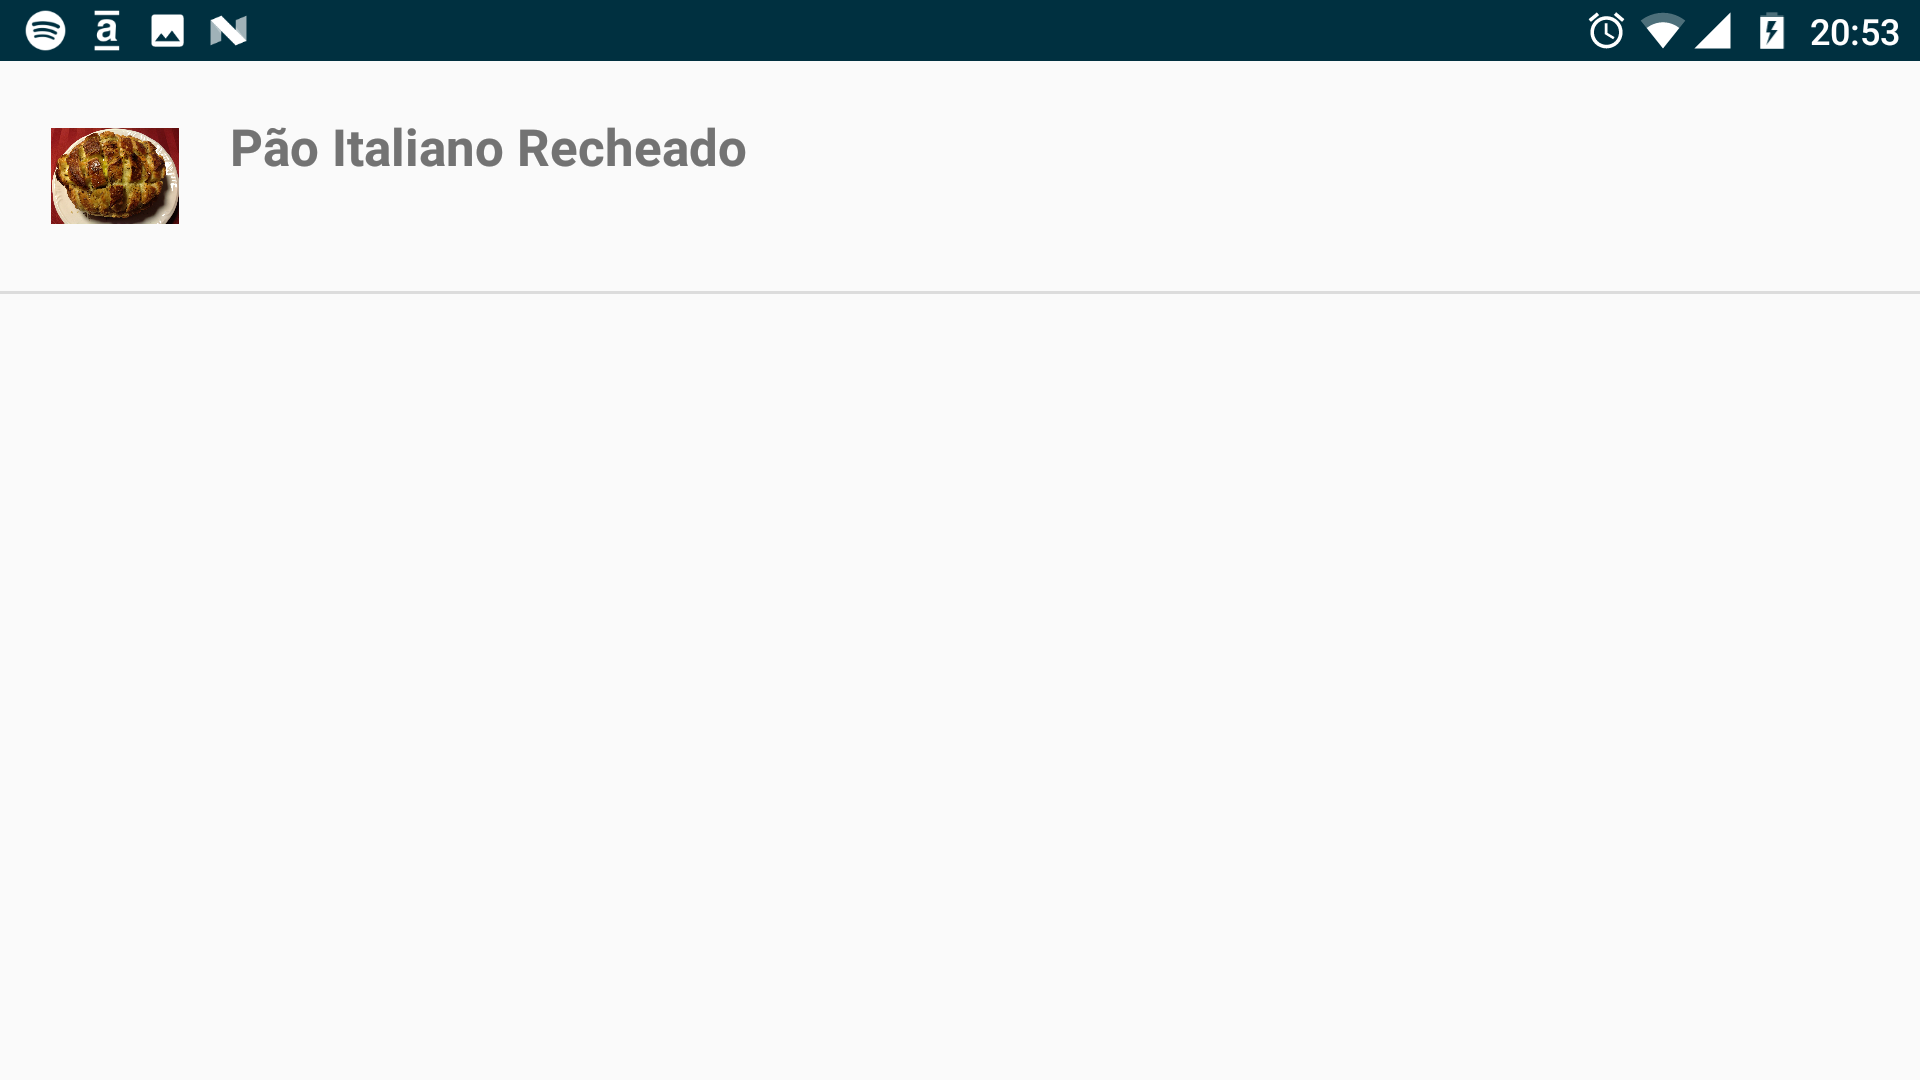
\includegraphics[width=0.8\textwidth]{cap5_rec_recipe_profile}
   
    \footnotesize{Fonte: Elaborado pelo Autor}
\end{figure}

Apesar de apenas uma receita ter sido sugerida, devido ao total de receitas muito reduzido do cenário, é possível validar a recomendação, já que está conta com o produto Queijo Mussarela.

\subsection{Alerta de Porta Aberta}

%% OBJETIVO
Os alertas ao usuário que esquecem a porta da geladeira aberta, ou não a fecham corretamente, é importante para evitar gastos desnecessários com energia e, possivelmente, com alimentos estragados. Como descrito na seção X, o processo de verificação de porta aberta, engatilha um registro no servidor. Considerando que, inicialmente, a porta estava fechada e, em dado momento, foi deixada aberta.

Após alguns segundos o seguinte registro foi feito na base de estruturas auxiliares, informando a situação.


%%%%%%%%%%%%%%%%% REGISTRO DE PORTA ABERTA  %%%%%%%%%%%%%%%
\begin{figure}[htb]
    \caption{Caption}
    \label{fig:cap5_open_door_reg}
    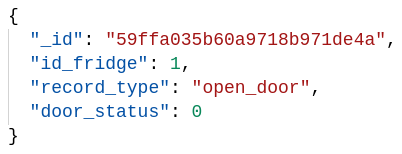
\includegraphics[width=0.5\textwidth]{cap5_open_door_reg}
    
    \footnotesize{Fonte: Elaborado pelo Autor}
\end{figure}

Algum tempo depois, a interface fez uma requisição ao serviço de estado de porta. Nesse caso, a aplicação da interface verificou que o estado era aberto e notificou ao usuário, conforme a Figura \ref{fig:cap5_open_door_alert}.


%%%%%%%%%%%%%%%%% IMG NOTIFICAÇÃO DE PORTA ABERTA  %%%%%%%%%%%%%%%
\begin{figure}[htb]
    \caption{Alerta de porta aberta}
    \label{fig:cap5_open_door_alert}
    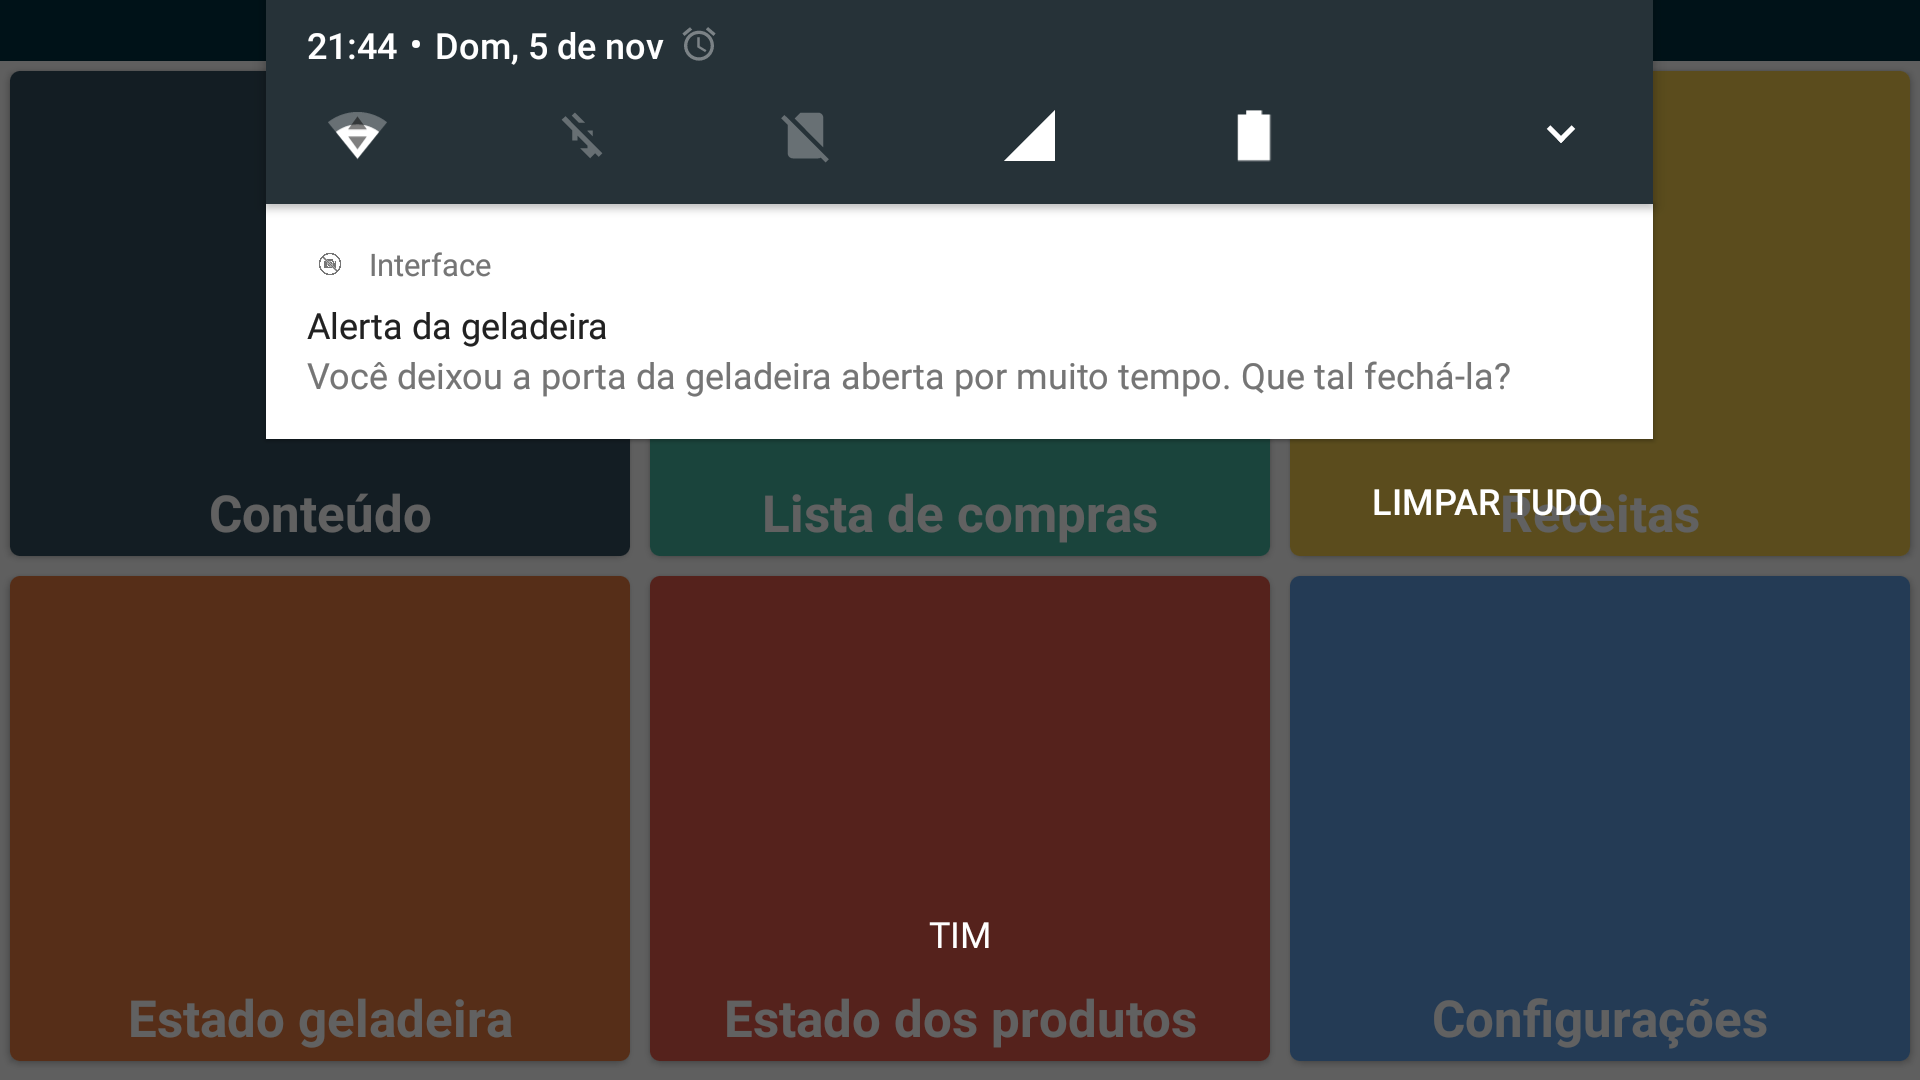
\includegraphics[width=\textwidth]{cap5_open_door_alert}
    
    \footnotesize{Fonte: Elaborado pelo Autor}
\end{figure}




